\documentclass{article}
\usepackage[english]{babel}
\usepackage{csquotes}
\usepackage{url}
\usepackage{comment}
\usepackage[a4paper, total={6in, 8in}]{geometry}
\usepackage{gensymb}
\usepackage{graphicx}
\usepackage{subcaption}
\usepackage{chngcntr}
\counterwithin{figure}{section}
\usepackage{tabularray}
\usepackage{xcolor}
\graphicspath{{./Figures/}}
\usepackage{float}

\usepackage[
backend=bibtex,
style=authoryear,
sorting = ynt
]{biblatex}
\addbibresource{Text.bib}

\title{My masters}
\author{Simen Storesund}
\date{\today}


\begin{document}
    \maketitle
    \section{Introduction}
    \textbf{Introduction} One baffling observation from the study of animal biology and neuroscience is how even seemingly simple animals are able to grossly outperform human-made robots, when animals operate with only limited spatial capability and the restraints of biological computations. This is true over a wide scale: not only are birds able to repeatedly and consistently trek thousands of miles between two locations each year, but a range of animal studies show how for instance mice flexibly and reliable learn to adapt to their novel environments, seemingly using a broad range of environmental cues to enhance their spatial understanding.
    Multiple studies have shown that mice navigate based on more than just experience - they are able to find novel shortcuts and navigate around new obstacles without much difficulty. This hints at the existence of some internal representation of the environment, which they can use to mentally compute possible paths to a destination, and somehow choose whichever path is best.
    [Maybe add some general observations about navigation, or other models for animal navigation here?]
    The transitional scale space model (TSS) seeks to explore how such a mental map would look, from a computational perspective \parencite{Waniek2020}. The model goes beyond spatial navigation, but the principles it operates under can easily be extended to a spatial environment, and posits, initially, that any model-based path finding system would require two separate memories: a mental map, or some internal representation of the environment, and some way to connect locations on this map together to get sequential routes between some start and some goal.
    While the physical space as experienced by mice is a continuous two-dimensional plane, any cognitive map of the environment must be represented by discrete neurons. This discretization of space could occur in many ways, but matching experimental observations, the TSS model suggests that this map could be a network of neurons in which each represents single locations in an environment. Part of the purpose of this network is storing information about each location, which is central for navigation: during path-planning, a mouse must be able to selectively avoid locations that are considered dangerous, which can be based on past experience of those locations. The cell in this map-network representing 'home' would elicit very different responses from the cell representing a dangerous territory, for instance if the mouse has encountered predators there previously.
    Such a network does not necessarily contain information about how locations are connected, spatially. Each node, or cell, in the network, does not know its own neighbors. This information is necessary for spatial navigation, and the TSS-model posits that this information can be stored in another network. In this network, each cell represents spatial transitions, to give information about which locations are available at a certain distance from a current location. However, due to the considerable number of possible spatial transitions, making each cell represent a single transition would require a high number of transitions, so the TSS model instead suggests letting each transition cell represent multiple transitions.
    The one constraint is that the network breaks down as soon as a transition cell represents a transition both to and from the same location - the domain of the transition cell, which are the places the transition cell transitions from, and the image, where it transitions to, must be disjunct. Apart from that, each transition cell should represent as many transitions as possible, to minimize the number of cells necessary in a working transition cell network.
    This argument stands at the center of the TSS model, because it posits that if a mouse brain indeed has these transition cells, they would be as efficient as they could be, appealing to the second level in Marr's three levels of analysis - in a biological network, any cell with a particular purpose should behave as to fulfill that purpose optimally, whatever the purpose is.
    Through mathematical derivations, the TSS shows that such a transition cell operating under the constraints listed above would have a striking spatial activity pattern. Although the mathematics won't be reproduced here, the logic behind an optimal transition cell is as following:
    a transition cell will be activated by all place cells in some limited region, referred to as a 'center' region, and will represent all transitions from that center to all place cells in a region surrounding this center, the 'surround' region. The transition cell will try to fit as many of these 'center-surround' regions into the environment as possible, as long as there is no overlap between center-areas and surround-areas.
    Indeed, in the limit of getting as many center-regions into the environment as possible, this transition cell will be active in a periodic, hexagonal pattern in an open environment, which is a solution derived from the sphere-packing problem in two dimensions \parencite{Waniek2018} [Cite sphere packing here?]. With optimal transition cells, all possible spatial transitions from center-areas to surrounding areas can be encoded in a network of only three such cells, highlighting how effectively these cells represent spatial transitions.
    A variable in these transition cells is the size of the center- and surround-areas, which in turn would influence the scale of the hexagonal activity pattern. A transition network as described in the TSS-model would work best with multiple separate scales, so larger scales can accelerate the retrieval of paths. In biological systems, where a transition cell has a rate coded activity in a gaussian for each center region, the ideal increment between scales is the \(\sqrt{2}\).
    On this basis, the TSS model predicts two memory structures in animals:  internal map, which consists of neurons representing single locations, and a network of transition cells trying to bundle as many transitions together without spurious transitions. Cells in the internal map-network should activate preferentially when the mouse is in some signature location, and cells in the transition-network should show a hexagonal firing pattern, representing available spatial transitions. This transition-network should also contain transition neurons on different scales, in which the increment from one scale to the next is the \(\sqrt{2}\).
    
    The following section will describe experimental results supporting and opposing these predictions made by the TSS model.
    Already fifty years ago, the place cell was observed in the mouse hippocampus, and this has led to a series of interesting experiments and observations \parencite{OKeefe1971,OKeefe1976}. Interestingly, the hippocampus was of interest because of its importance in episodic memory formation. The canonical hippocampal pathways divide the hippocampus in three regions that communicate in a feedforward manner: the dentate gyrus receives inputs from outside the hippocampus, and project these to CA3, which both has recurrent excitatory connections as well as projections to CA1 [Source here?]. The main output region from CA1 is the subiculum, which is outside the hippocampus and projects to the prefrontal cortex. Place cells have both been observed in CA3 and CA1, but have not been seen outside the hippocampus.
    The place cell typically fires with a rate that is distributed in a gaussian around one or a few locations in the environment, so a network of place cells can encode all positions in an environment \parencite{Wilson1993}.
    One line of evidence that suggests that place cells participate in navigation is sequential activity, observed both during and after navigation. Sequential place cell activity during rest or sleep after navigation, called replay, reflects both sequences of place cells in the order they were active during navigation, or reverse sequences \parencite{Wilson1994}. Interestingly, replay occurs during sharp wave ripples, in which the place cell activity is temporally compressed relative to their activity during navigation.
    Preplay refers to sequential place cell activity during navigation. During preplay, place cells corresponding to the current location is followed by place cells that will be active a short time into the future, indicating that the hippocampus has some information about upcoming place cells \parencite{Dragoi2011,Dragoi2013}.
    The hippocampus is also subject to oscillations in the local field potential, prominently in the 4-11 hZ region, called theta oscillations, or just theta. When preplay is viewed relative to theta, the place cells corresponding to the current locations are active at the trough of the wave, while past place cells activate in the descending part of the wave, and future place cells activate in the ascending part of the wave. This phenomenon is called theta wave precession (Mosers and Hafting on grid cells, someone else on place cells?).
    Replay typically occurs during rest or sleep following explorations, in which sequences of place cells experienced prior to rest are activated again, but compressed temporally (Tonagawa)\parencite{Olafsdottir2016} . Moreover, combinations of sequences are seen, which seems to produce novel trajectories in an already explored space.
    Interestingly, place cells can be active in multiple environments, but they remap independently of each other (O’Keefe, other sources here?). This implies that the place cell networks are modulated by the context, but the mechanisms for this are currently unknown.
    Grid cells were originally found in the search of afferents to the hippocampus place cell system, first found in layer II of the medial entorhinal cortex (mECII)\parencite{Hafting2005}. Grid cells are characterized by periodic spatial activity, arranged so that the firing fields make up hexagonal patterns spanning the environment, and this activity is found both in stellate- and pyramidal cells of mECII(Hafting, or someone else?). These cells are also firing independently of head direction or velocity, and have since been found in multiple other parts of the brain, such as in deeper layers of the medial entorhinal cortex (III - IV), as well as the pre- and para-subculum (Cite these here).
    Grid cells, too, have received a lot of attention, and a series of details about their firing properties has since been revealed. Grid cells seem to align with the boundaries of their environment with a small wall-angle offset, and grid cells located near each other in the entorhinal cortex also share the spacing, or size of each hexagon (Some other sources here?). However, along the dorsoventral axis, the spacing of the grid increases by a factor of the square root of two (Also, source?). Grid cell activity is strikingly robust across trials and time, and it also seems to persist when visual cues are removed (Source). However, their hexagonal gridness depends on the environment shape, and their firing pattern gets distorted in trapezoid or not-regular environments \parencite{Stensola2015,Krupic2015}.
    Grid cells also exhibit theta wave precession during navigation \parencite{Hafting2008}, and interestingly, when abolishing the theta rhythm by lesioning the medial septum, grid cell activity loses their spatial correlation in mice, so theta rhythm seems critical for the grid cell pattern (Brandon, 2011, and Koenig, 2011). However, this was not seen in similar experiments in bats \parencite{Yartsev2011}.
    Typical input regions to the medial entorhinal cortex are the post- and perirhinal cortices, as well as the pre- and parasubiculum, which seem to integrate information from multiple sensory modalities, but to the author's knowledge, the concrete input structure to grid cells is not known (Multiple sources required here, lol).
    Within mECII; grid cells seem to be interconnected by parvalbumin-positive interneurons, applying strong, lateral somatic inhibition, while excitatory connections have not been observed \parencite{Couey2013,Buetfering2014}. Moreover, maturation of this interneuron structure seems to reinforce and strengthen the spatial correlations of grid cells \parencite{Christensen2021}. 
    Connectivity between grid cells and place cells are only partially mapped, but in addition to the canonical tripartite synapse model, which understood the dentate gyrus as the main input region of the hippocampus, the mECII also projects directly to CA1 (Check Witter’s review, find sources there). This suggests that place cells might be formed based on summation of grid cell inputs on multiple scales, but this idea was contradicted when it was found that place cells mature earlier than grid cells in development (postnatal day 16-17 versus postnatal day 19-20) \parencite{Langston2010,Wills2010,Wills2012}. However, it has been established that CA1 also projects strongly back to mECII, and that grid cell activity depends on these connections \parencite{Bonnevie2013}.
    A multitude of models and model families already exist to explain the wealth of experimental data on grid cells, with differences in their suggested mechanisms for the grid pattern, as well as the purpose of the grid cell. Due to their persistent spiking in darkness, many models assume that grid cells do path integration, integrating self-movement information to predict current location in the absence of external inputs(Hafting, plus a bunch of models, or a review?). Oscillatory interference (OI) - models seek to explain the theta phase precession in grid cells, and have shown that grid-like activity can be achieved by the interference of multiple oscillators in membrane potential \parencite{Burgess2007,Zilli2010}. The OI-model can account for many activity patterns, but if the different oscillators differ in frequency by a sufficiently small margin, and adapt this margin based on speed- or velocity-signals, the cell can have a grid-cell-like activity with spacings as observed in experiments. Also, these methods effectively explain the phase precession observed in grid cells. 
    Another set of models explain the grid cell as a part of a continuous attractor network (CAN), which can explain persistent grid cell activity during rest or sleep \parencite{Yoon2013,Widloski2014}. These models can be implemented with lateral inhibition between grid cells, as observed in mECII, as long as the strength of the inhibition is inversely proportional to the overlap of firing fields, so the most active grid cell silences all other grid cells. When the animal moves, this activity is shifted to a grid cell with a neighboring phase.
    It has been demonstrated that any such system of path integration still needs regular external input to avoid drift, and the exact inhibitory structure predicted by CAN - networks have not been observed. Additionally, the velocity-based inputs have not been observed, although this might just stem from the unexplored input-space of grid cells (Some review claimed this).
    A third set of models predict that grid-patterns can be learnt by Hebbian mechanics, or by associating to the right spatial inputs and dissociating to other spatial inputs. Early methods found grid-like activity with neurons experiencing firing fatigue, and subsequent models have produced grid cells purely with spatial inputs. For instance, (Castro and Aguiar) showed that grid cells can occur from place cell inputs, and (Mercado and Leibold) made a model with center-surround inputs from place cells, arguing that grid cells is some turing pattern learnt on top of a place cell network. 
    It is this third set that is the most similar to the TSS model, because grid cells are not assumed to rely on velocity-signals to perform path integration. In the TSS model, the suggested mechanism by which transition cells learn is suggested to be similar to how place cells learn their receptive fields. The place cell learns to activate based on spatially modulated sensory inputs, in which each place cell associates to spatial inputs from one area, and lateral inhibition prevents other place cells from activating. This has been explored in numerous works prior to TSS, for instance using boundary vector cells or object vector cells as inputs \parencite{Barry2006}(am I correct saying this also exists for OBCs?). Boundary vector cells and object vector cells are similar in that they activate preferentially when the animal is at some distance and direction relative to an external structure. Cells are called boundary vector cells if this structure is an environment boundary, such as a wall or a cliff, while they are called object vector cells if the structure is some environment landmark. Using cells like these as spatial input in a feed-forward network is attractive because the cells can plausibly exist and be configured prior to exploration, and computed during exploration through optic flow \parencite{Raudies2012}.
    Under the TSS-model, grid cells, which are suggested transition cells, are also formed from spatially modulated inputs. As opposed to place cells, these associate to spatial inputs in center-regions, and dissociate to inputs from the surrounding-regions, while trying to fit as many center-regions into the environment as possible. These transition cells are also interconnected by strong lateral inhibition, to discourage overlapping center-regions.
    Notably, the TSS-model only assumes this learning rule for the lowest transition-scale, while subsequent scales can be learnt from inputs on the last scale.
    This learning rule has been proven in discrete-time simulations in networks of three transition cells, which received spatial inputs sampled from a regular, rectangular grid of spatial cells. However, the simulations did not produce grid cells with more than three transition cells, and it is unlikely that such an input-network of regularly distributed place cells actually exists prior to exploration. Both of these constraints need to be addressed for this learning rule to carry biological plausibility, in which any transition network probably would consist of more than three cells, possibly with overlapping center-areas, and in which the input-structure should be reasonable in a novel environment.
    In this work, the main objective is to establish this network structure in a more biologically plausible way, and explore under what conditions or constraints transition cells develop a hexagonal structure. The two main subgoals is to first see if a biologically plausible network can contain more than three grid cells, by simulating in continuous time to see if delayed inhibition can allow overlapping grid fields.
    Secondly, the way the structure of spatial input affects gridness is also explored. To allow for a center-surround learning rule, spatial input was always phase-coded, so the grid cells received pulses of inputs in simulated theta-cycles, in which the more relevant inputs arrived earlier, and a STDP-learning rule separated center from surround input. For highest biological plausibility, this input would be boundary vector cells or similar, and this was attempted with complex dendritic computations to allow differentiating vector-inputs, but place-cell like distributions were also attempted to reduce the simulation complexity and simulation times. With a simple STDP- based learning rule, robust gridness scores were observed with multiple network structures, showing that cells can learn spatial transitions effectively under biologically plausible conditions.
        
    \section{Methods} 
    \subsection{Overall model design and -goals}The purpose of this thesis is to test gridness in transition neurons as described by the TSS-model with biologically plausible spatial inputs and conditions (continuous time). To achieve this, transition cells were simulated in a spiking neural network, which are artificial networks with certain properties:
    \begin{enumerate}
        \item The network is simulated with continuous time, or in time steps that are significantly shorter than the mean firing rate of neurons.
        \item Neurons communicate in temporally discrete spikes, triggered when an internal voltage variable exceeds a threshold.
    \end{enumerate}
    
    Different network structures have been tested over the course of the thesis, and the results of different structures are treated in the results section. This section will first describe an ideal network, and describe the different assumptions that network would operate under. Further sections will describe other network structures that were used to simplify and test different levels of plausibility.

    An ideal network has the following properties: it is simulated in a biologically plausible network, such as a spiking neural network. Most importantly, this means that communication happens at a delay, time is continuous and learning rules must be online and local. Simulations get inputs from some plausible spatially tuned neurons, more precisely boundary vector cells (BVCs), whose activity is based on real or simulated trajectory data. From these inputs, another layer of cells of arbitrary size learns center- and surrounding area information to represent transition-cells as described in the TSS-model, encoding transitions on a single scale. Under these constraints, the objective is whether the transitional neurons self-organize into single-cells with hexagonal activity patterns in space, and in which the population covers all possible environment transitions.

    Both an ideal network and subsequent simplifications will have some common features to accommodate these limitations: first, spike timing dependent plasticity is a biologically plausible learning rule which both allows single transition cells to associate with spatial inputs associated with center, and dissociate with inputs associated with surround areas. To facilitate this, all inputs arrive in pulses at theta-wave frequency, 10 Hz, in which only spatial input with sufficiant relevance is active. The input is also phase coded, so the less relevant, the higher the temporal offset is relative to theta. This means that a transition cell is likely to fire following center-inputs, and subsequently receive a burst of inputs from cells representing surrounding locations. The STDP learning-rule will ensure that the center-activity which arrived pre-spike are potentiated, and the surround-activity arriving post-spike is depressed. Secondarily, all active inputs are slightly potentiated to encourage the transition cell to be active in as many center-areas across the environment as possible.

    \begin{figure}[H]
        \centering
        \begin{subfigure}[][][c]{0.6\textwidth}
            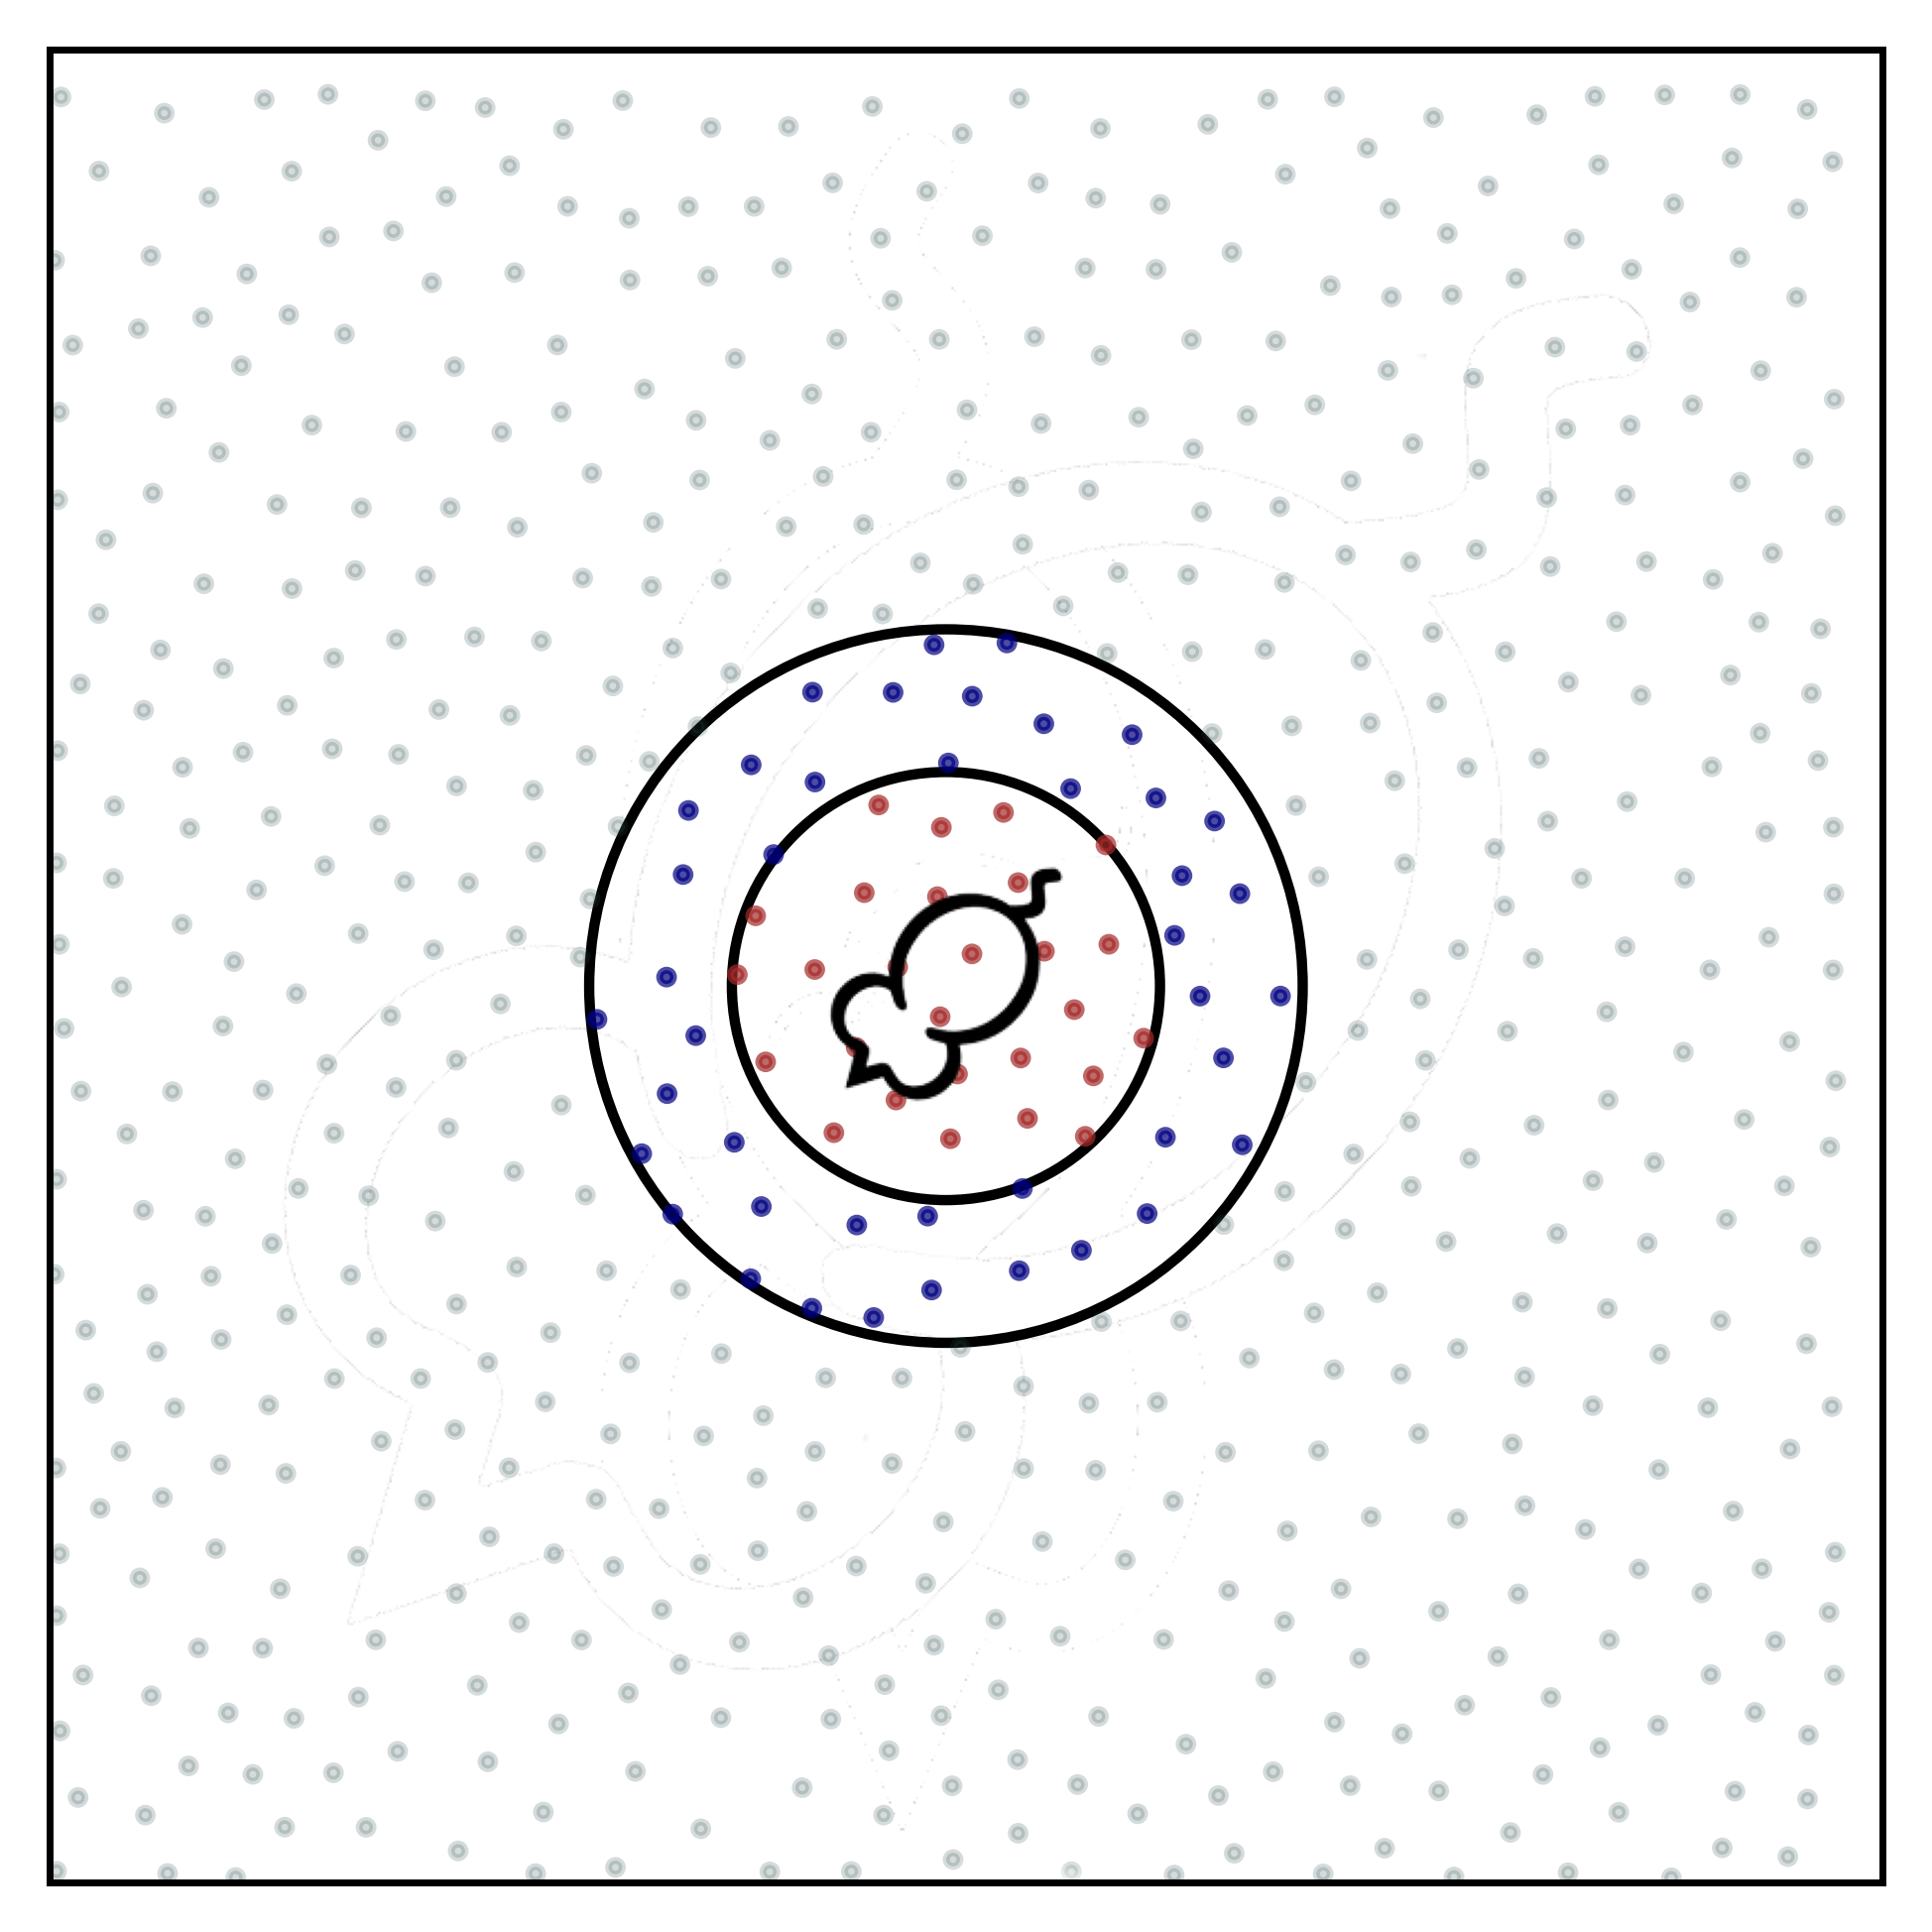
\includegraphics[width = \textwidth]{mouse_plot.png}
        \end{subfigure}
        \hfill
        \begin{subfigure}[][][c]{0.33\textwidth}
            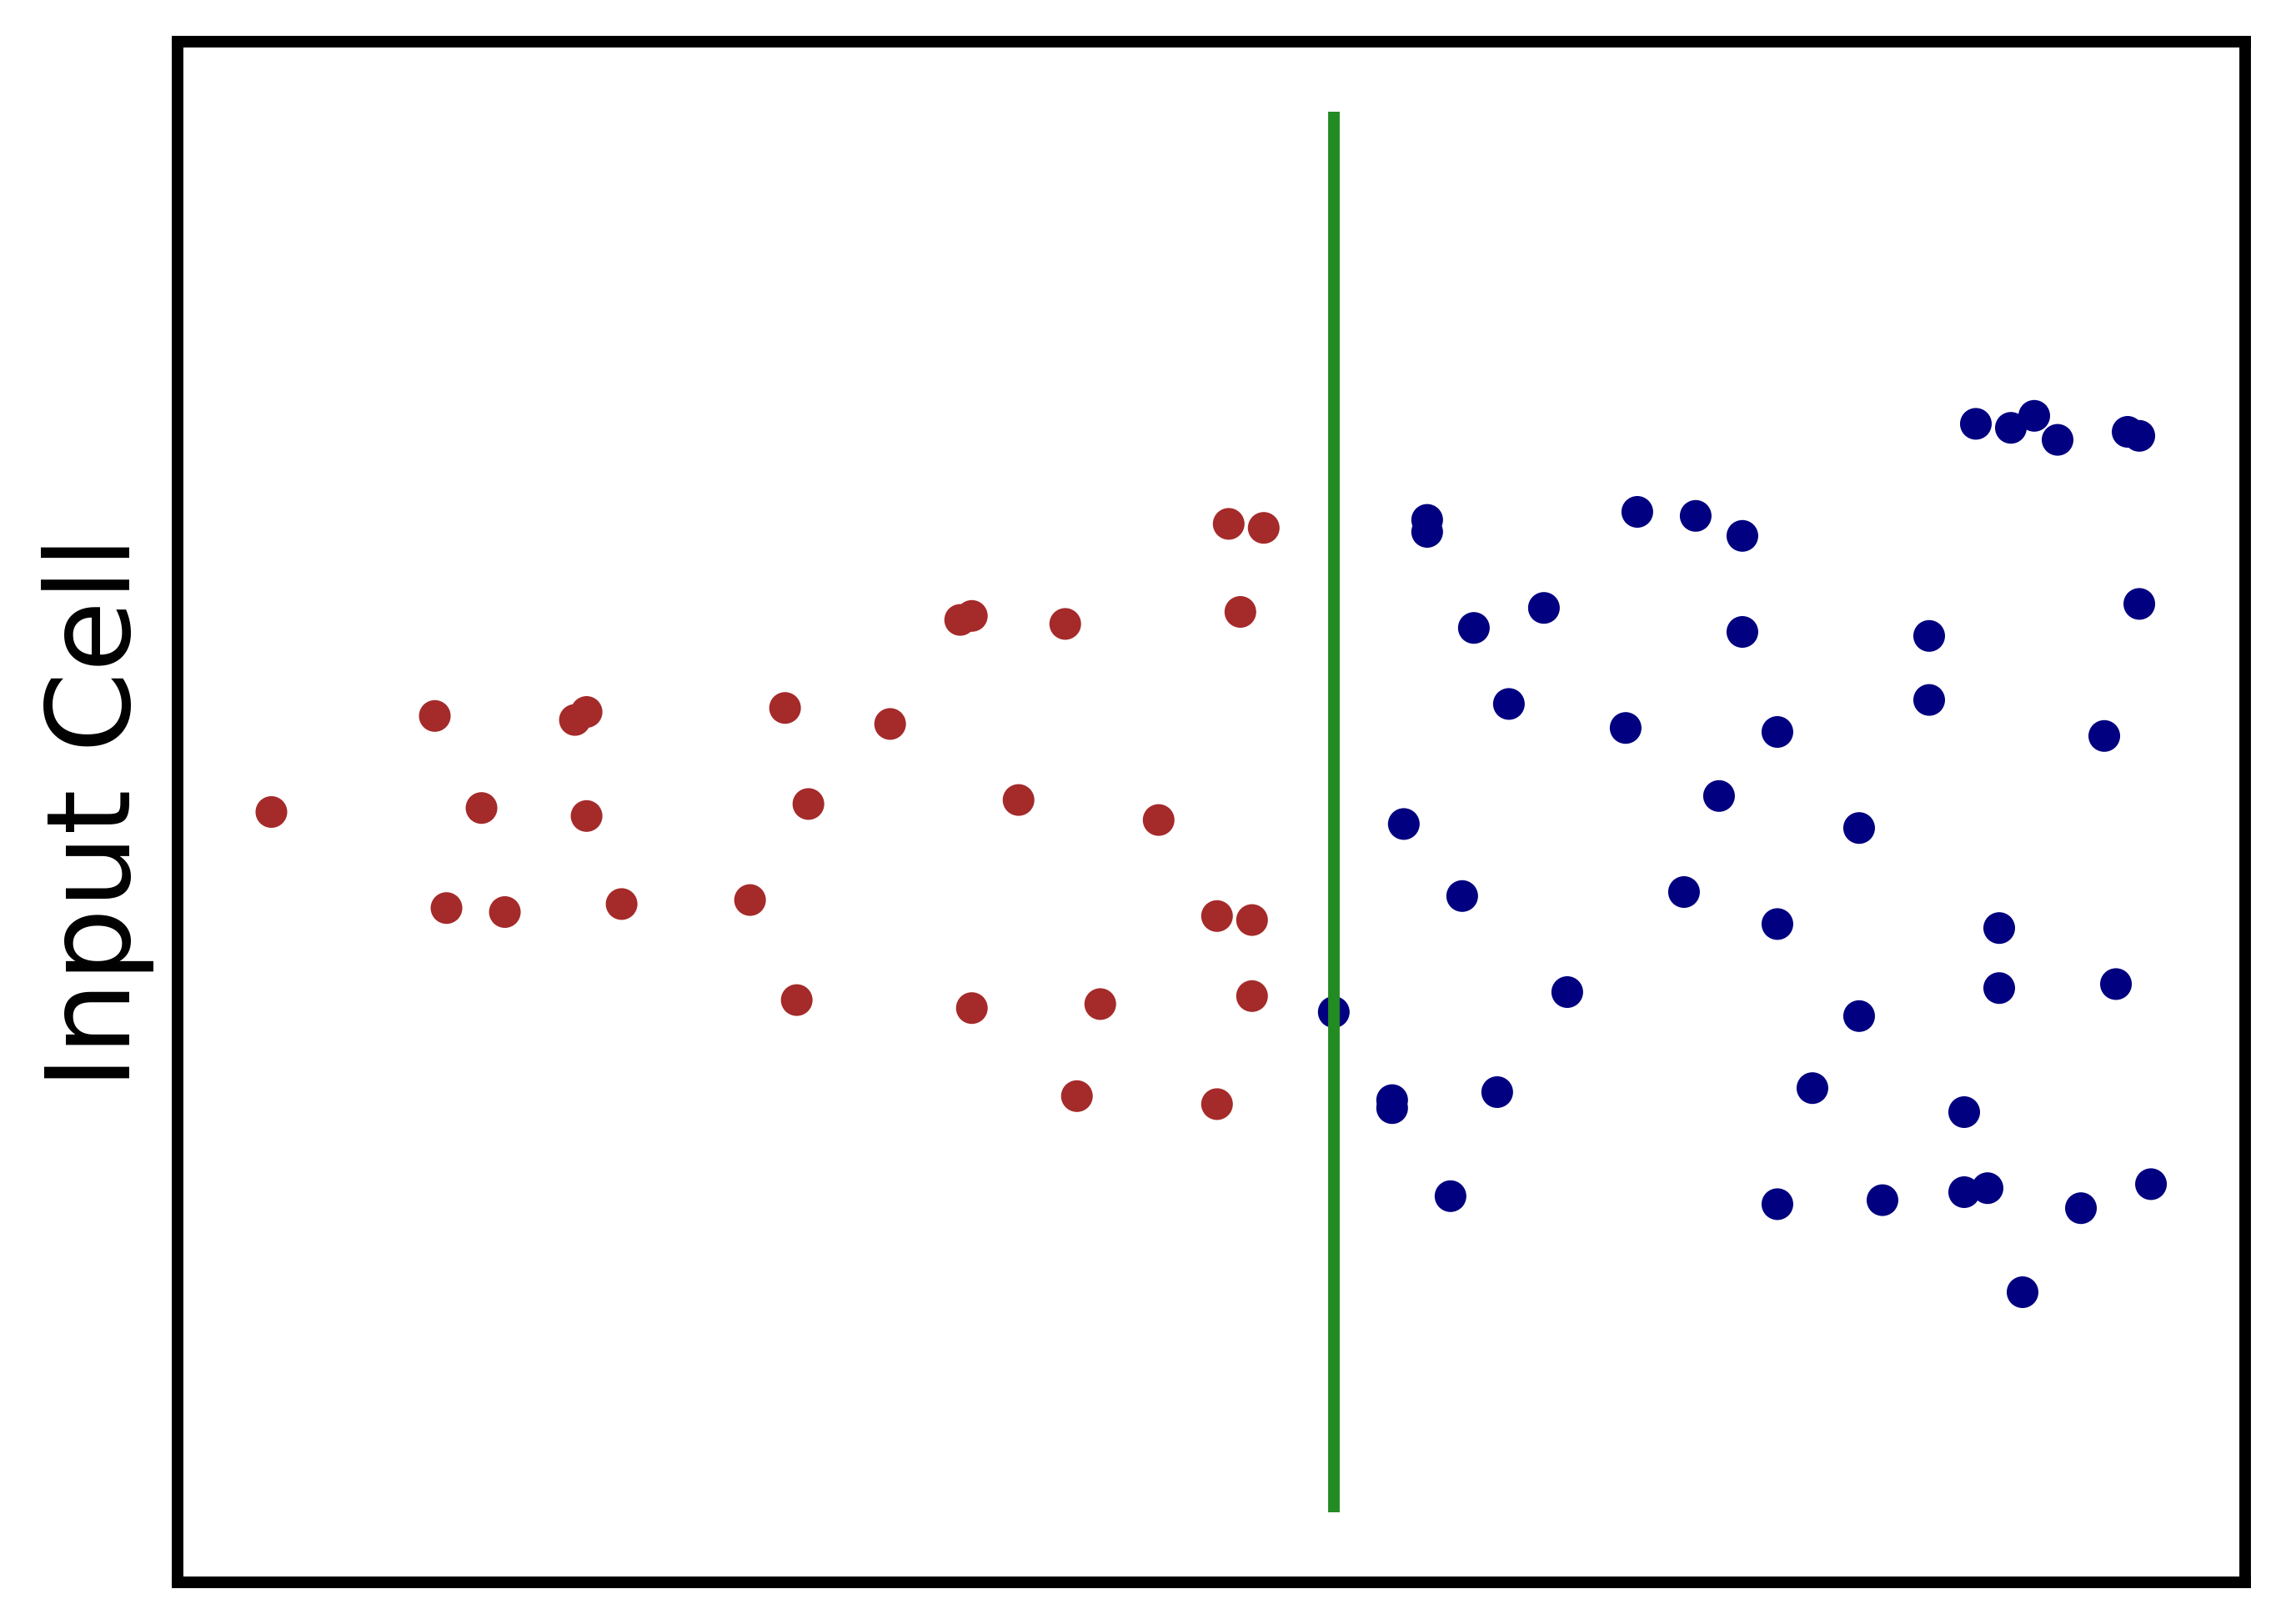
\includegraphics[width = \textwidth]{input_STDP_plot.png}
        \end{subfigure}
        \hfill
        \begin{subfigure}[][][t]{0.33\textwidth}
            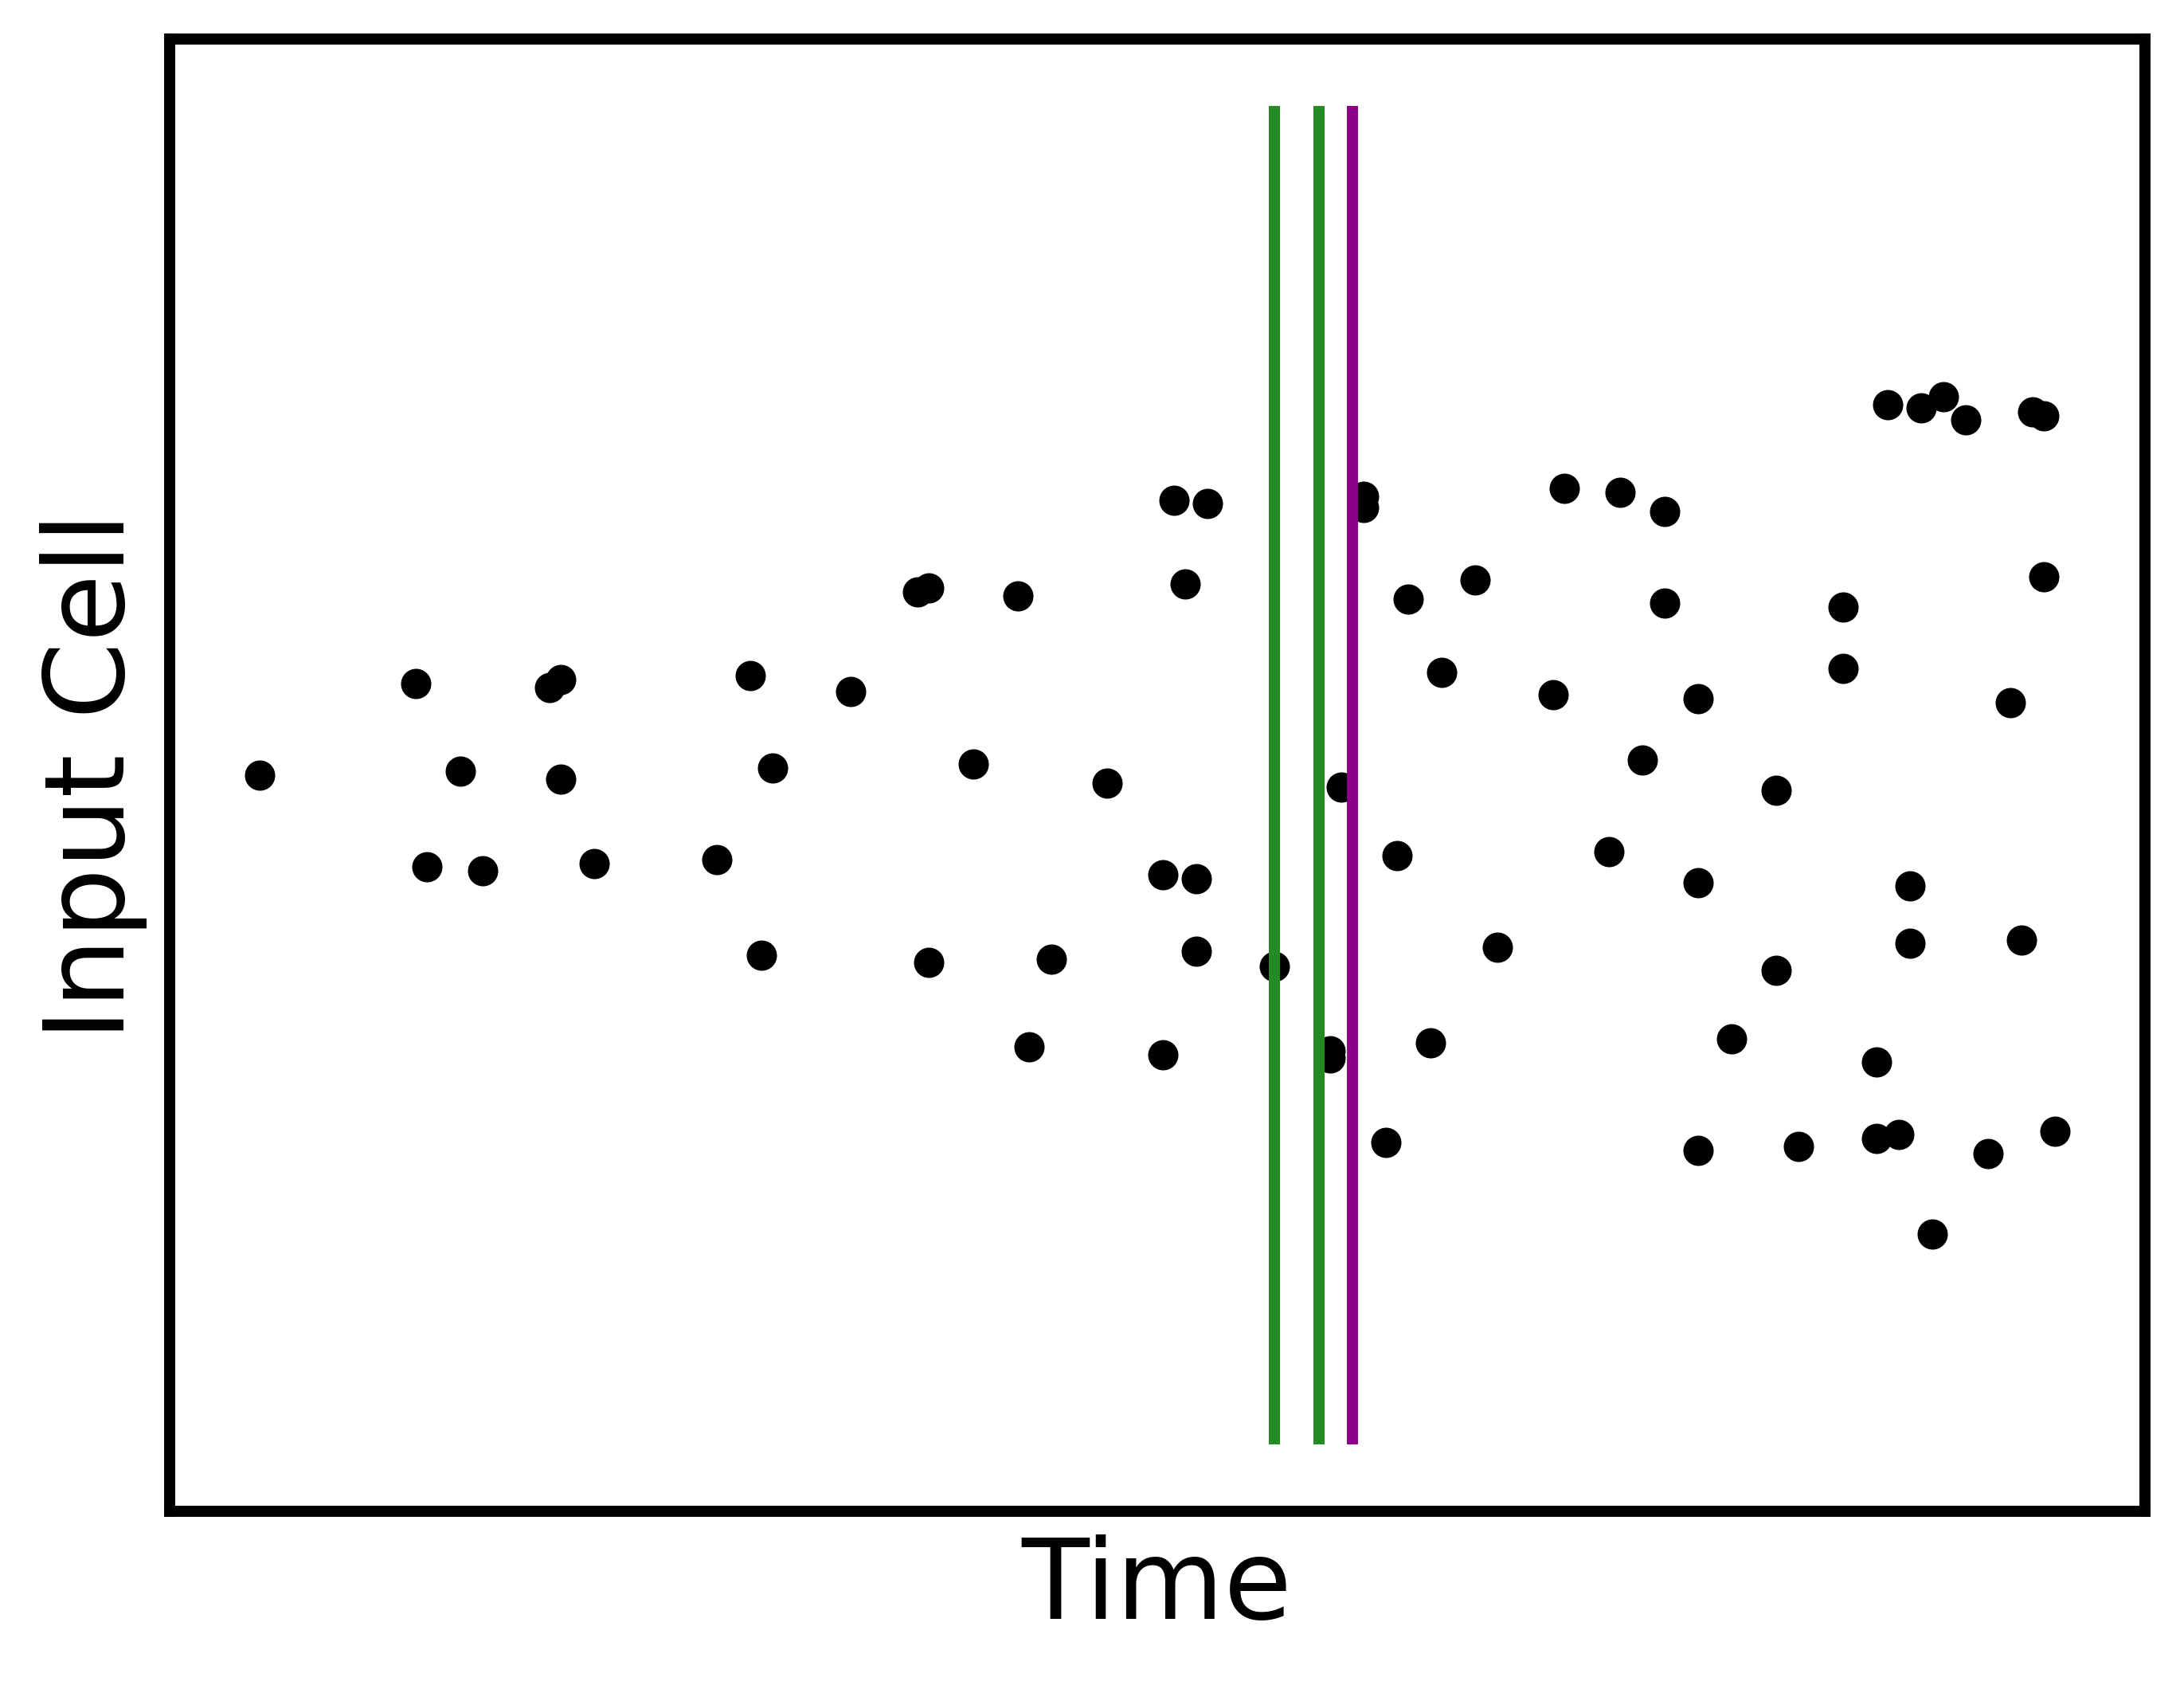
\includegraphics[width = \textwidth]{input_inhibit_plot.png}
        \end{subfigure}
        \begin{subfigure}[][][b]{\textwidth}
            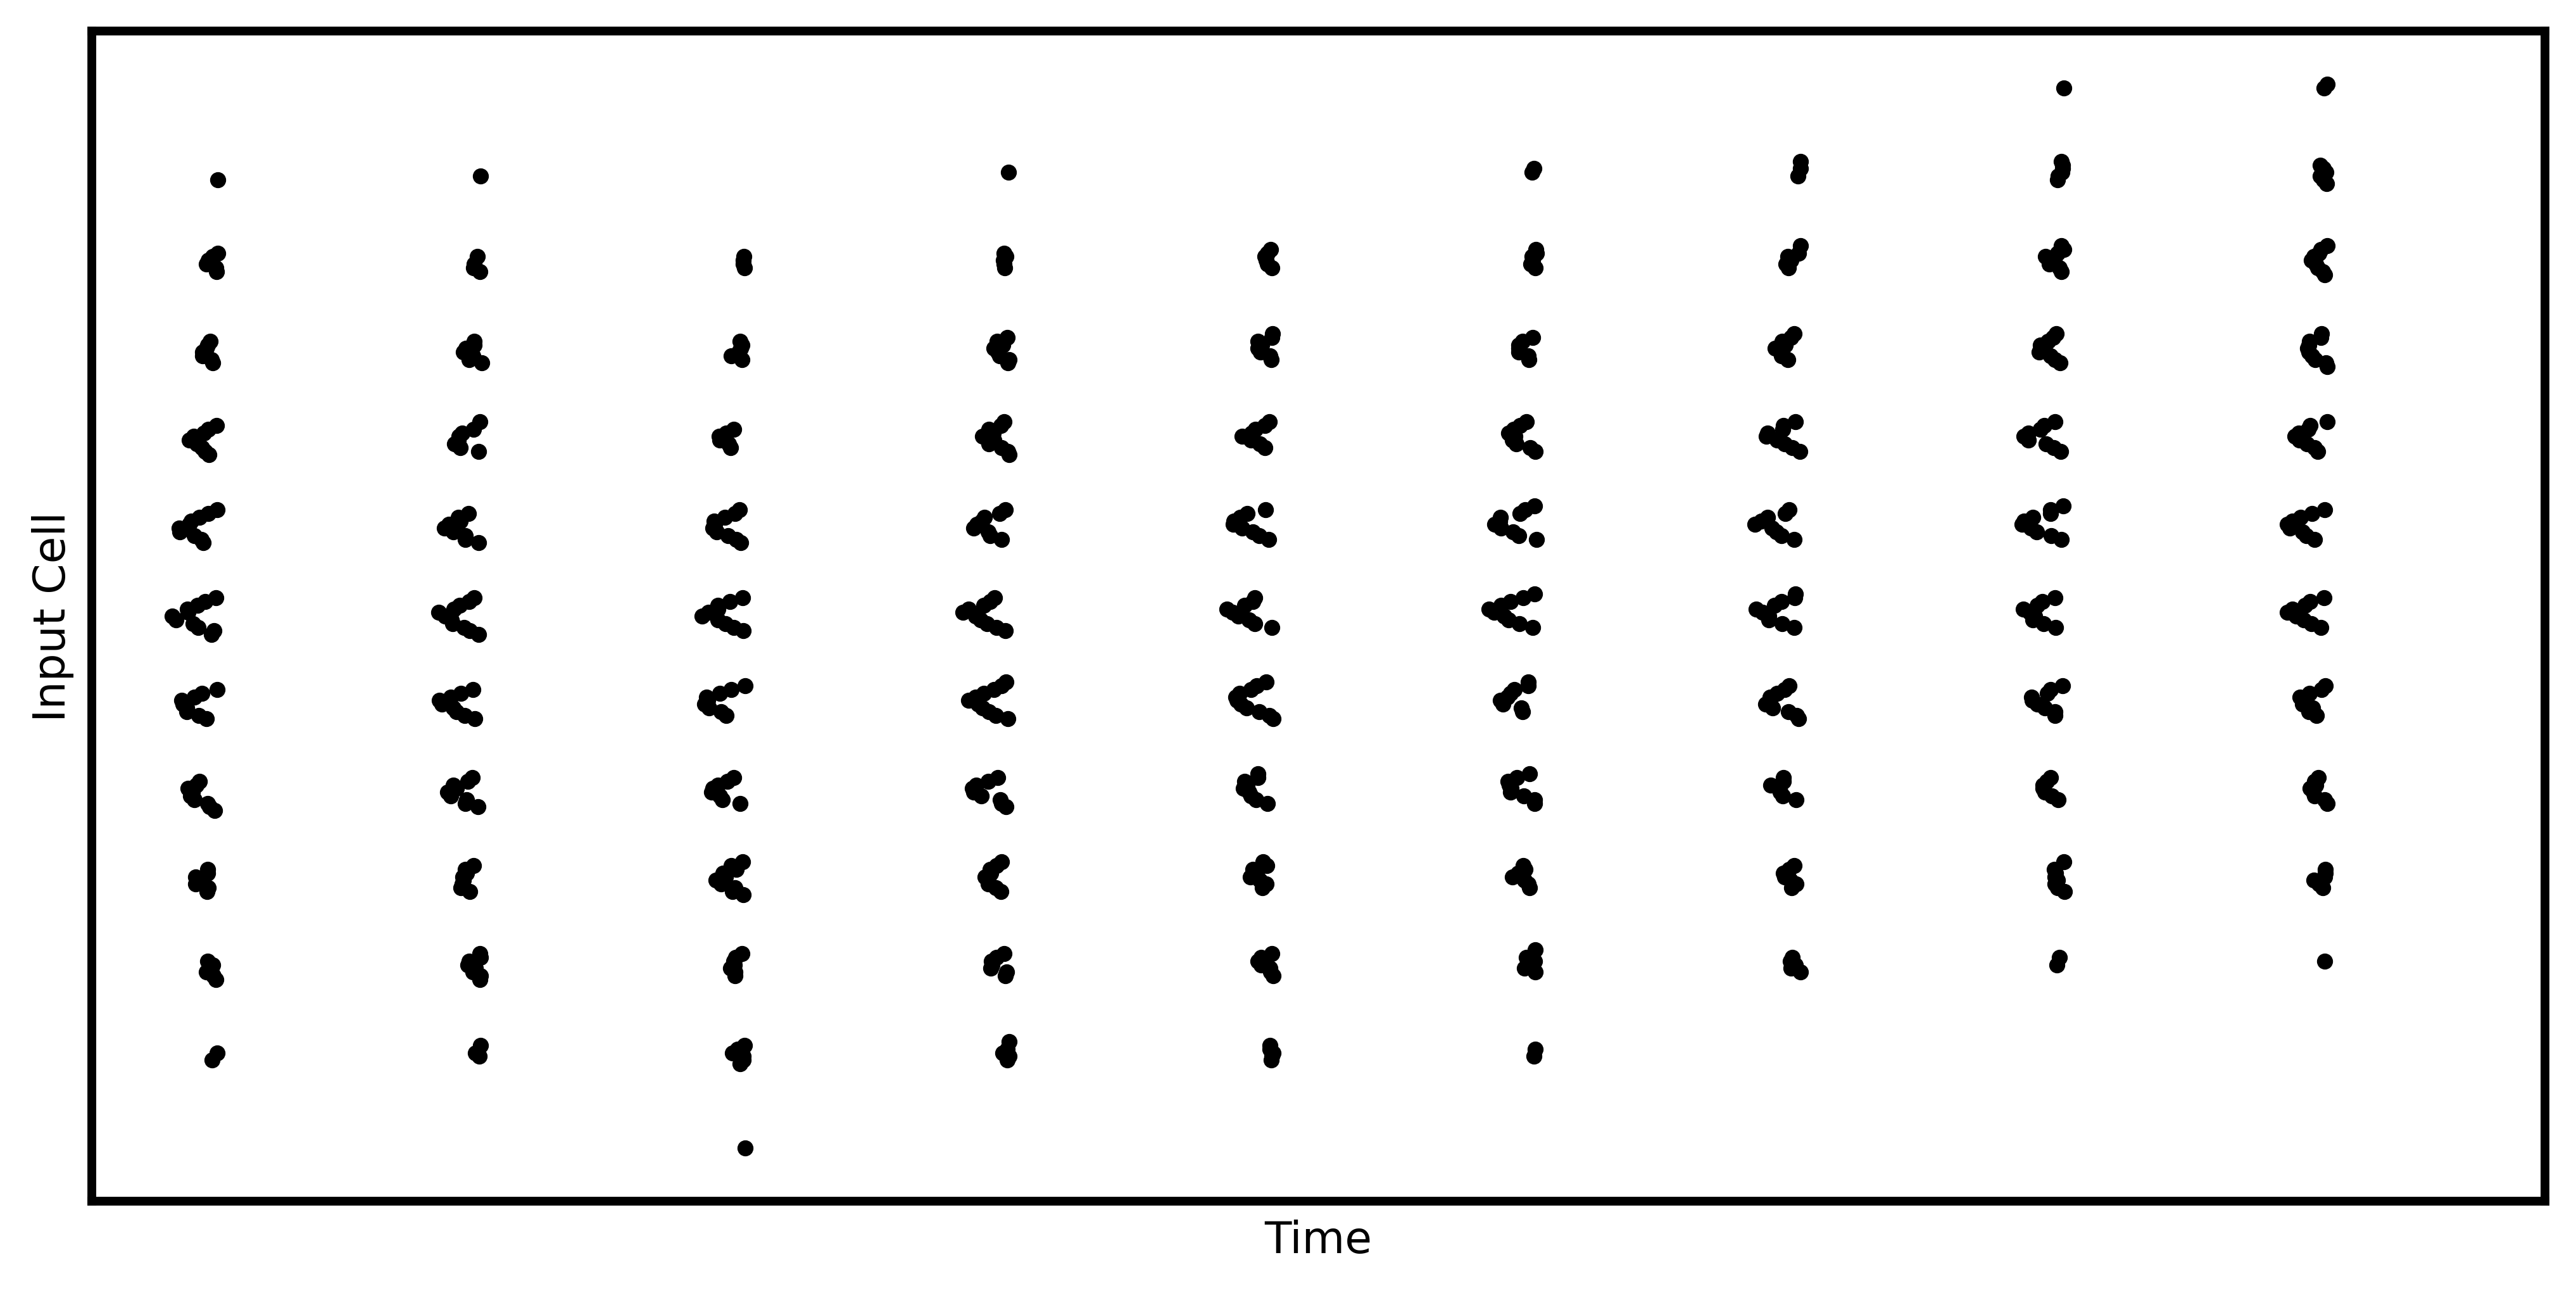
\includegraphics[width = \textwidth]{input_plot.png}
        \end{subfigure}

        \caption{Spatial inputs from a region surrounding the mouse will be activated each theta-cycle, here shown as inputs within the two surrounding circles. This input is phase-coded, so cells responding to locations nearest to the mouse will arrive earlier. With a STDP learning rule, this can lead to association to the central inputs, and dissociation of the surround inputs, as shown by the innermost surrounding circle.}
        \label{mouse_plot}
    \end{figure}

    
    An inhibitory layer connects transition cells laterally, causing strong inhibition, but on a delay. This leaves a narrow window in which multiple transition cells can fire, followed by complete inhibition, so some transition cells partially associate to the same areas.

    Due to the high number of parameters available in such a network, the network would preferably see characteristics of the transition cells, such as grid-patterns, emerge quickly and without perfectly honing parameters.
    This is both because a network structure that produces grid cells only with very particular parameters is less biologically plausible, and because testing the parameter space properly is time consuming. On this note, there are reasons to think that a network in which grid cell activity occurs in transition cells based on linear summation of BVC input, as shown in figure 2.1, is difficult to achieve. For one, boundary vector inputs in neighboring areas are typically highly linearly correlated, so the transition cell would struggle to associate to one location and dissociate from a neighboring one. Secondly, for instance in square environments, one could imagine picking two locations that the transition cell has associated with, denoted \((x_1, y_1)\) and \((x_2, y_2)\). In locations \((x_1, y_2)\) and \((x_2, y_1)\), the input would be highly similar to half the input from position 1 and half the input from position 2, but the transition cell should not fire in these locations, because that would lead to rectangular-grid firing patterns, not hexagonal. It should be noted here that the spiking neural network itself implies non-linear features that might have enabled such a network to produce grid-cells. One way to achieve this would be with other transition cells that are sufficiently active in location \((x_1, y_2)\) and \((x_2, y_1)\), so they inhibit the first transition cell. However, due to the fine-tuning such a network would require, this network structure was not pursued further.

    An appealing alternative, which highlights the advantage of biological neurons, was to consider nonlinear dendritic computation on transition cells in a multi compartment model. Under this idea, although boundary vector cells technically synapse onto transition cells directly, the simulation treats dendrites as separate units within one transition cell. Each dendrite would get inputs from some subset of BVCs, and the transition cell can associate and dissociate to all inputs on an entire dendrite. Similarly to the BVC-model, each dendrite would preferably be active in only single locations in the environment, for instance by responding non-linearly to inputs with a soft-max activation function (as in the other paper). In the example above, this would let the transition cell associate to dendrites responding highly to \((x_1, y_1)\) or \((x_2, y_2)\), while remaining dissociated from dendrites activated in \((x_1, y_2)\) or \((x_2, y_1)\), without sacrificing biological plausibility. This multi compartment model satisfies all requirements stated above. 

    However, to shorten simulation time and reduce complexity, this kind of network can be simplified. This can be done incrementally, in which each step simplifies complexity but also reduces plausibility:
    \begin{enumerate}
        \item The BVC-model showed that place-like activity can be produced from BVC-inputs. As such, BVC-input can be replaced by place-like inputs directly as non-spiking dendrites in the multi-compartment model. 
        \item To reduce the number of neurons, each dendrite can connect to each grid-cell, and the dendrites can be spiking to reduce computational time for each of them. Here, the dendrites still fire in random places, according to some distribution.
        \item The dendrites can respond to places distributed in a regular, rectangular grid.
    \end{enumerate}
 
    Note that step 3 is highly similar to the already existing simulations by Waniek (citation?), just here in a spiking neural network. This was useful, because it allowed testing the hypothesis that transition cells can produce grid-like behavior in networks of more than three neurons if the inhibition is delayed, not showed in previous simulations. Then, networks could gradually be made more complex and biologically plausible, leading to a series of networks that could be tested sequentially from simple and less plausible to more complex and more plausible. The concrete implementation of each network and other considerations are treated in their own upcoming subsections.

    \subsection{Simulation software} All models and implementations can be found on github(Insert link here?), and while the simulation data is not available on github due to storage capacity, it is available (somewhere else?). All simulations were implemented in python, using the brian2-library for its flexibility and easy implementation (cite brian2 here). Simulations used artificial trajectories, either simulated by an algorithm written by Waniek (how should I describe this - refer to sources on mouse trajectory data?) or using RatInABox  to also extract boundary vectors for BVC-inputs (cite ratinabox here). Spatial inputs were calculated prior to simulations, using either position-data or boundary-data from the trajectories, and added to a brian2 spikeGeneratorGroup. The network state was stored frequently during simulations, so the network-states could be reconstructed later for resampling. 

    \subsection{Rectangularly spaced inputs} This network structure is heavily inspired by previous TSS-simulations, with three layers: input neurons, transition cells and inhibitory neurons. The input neurons have a preferred spatial location, and have the chance of being activated each theta cycle, which is set to happen with a 10 Hz frequency. The activation function for input neuron \(i\) with position \((x_i, y_i)\) is \begin{equation} \label{key1} delay = \frac{\sqrt{(x_i - x)^2 + (y_i - y)^2}}{\sigma} + \mu\end{equation}
    in which x and y is the current location, \(\sigma\) is a scale parameter determining the width of input, \(\mu\) is noise and delay ends up in ms. Typically, there was a cutoff at 20 ms, so only reasonably active inputs would activate, but this cutoff was arbitrary. Each of these inputs synapsed on each transition cell, with weights randomly drawn from a uniform distribution between 0 and some maximum, \(w_{max}\). The transition cell had a voltage parameter which triggered spikes if it surpassed a treshhold, or updated according to the formula: \[ Insert formula here: I don't know how to get this into a single thing...\].
    The STDP learning rule was implemented by separating potentiation and depression: upon transition cell firing, potentiation for weight \(i\) worked according to the formula \begin{equation} \label{key3} w_i = clip(w_i + a^{pre}_i \cdot \nu, 0, w_{max})\end{equation} in which \(a^{pre}_i\) is a variable incremented when input \(i\) fires, and decays with time. \(\nu\) is here a learning rate, which can be constant or variable. 
    Similarly, upon presynaptic input from input \(i\), weights are depressed, but also increased according to a baseline parameter, according to \begin{equation} \label{key4} w_i = clip(w_i + (a^{post}_i + \alpha \cdot (w_{max}-w_i)) \cdot \nu, 0, w_{max})\end{equation} where \(a^{post}_i\) is a symmetric parameter to \(a^{pre}_i\), but which decrements upon post synaptic firing and decays at a separate rate. The baseline weight increase operates with rate \(\alpha\).
    Transition cells then interact by activating inhibitory neurons which inhibit all transition cells for a time, typically by reducing their voltage by a large, constant amount, but which is small enough so the voltage returns to zero by the next theta.
    In this model, all synapses were given a delay, but the feedforward nature of inputs to transition cells made the delay here redundant.

    \subsection{Randomly spaced inputs}
    This network structure had similar structure and learning rule to the network in the section above. In these networks, however, there is some randomness in determining which area an input neuron responded to. This was implemented in three categories: one, the inputs were first arranged in a grid, and then randomly jittered slightly in some random direction. Two, the inputs were distributed in a blue noise like pattern, to ensure a relatively even, although not regular, distribution of spatial firing. Three, the inputs were distributed in a white noise like pattern, in which one input neuron would respond to areas independently of other areas.
    While inputs responding to areas in a uniformly random, independent manner would be the easiest, from the perspective of BVC-to-transition cell inputs, it brings the possible disadvantage that some areas will be less covered, so a transition cell that's supposed to fire in some region according to its grid might not receive any input there at all.
    Inputs that were regular, but jittered, were generated by first generating regularly spaced inputs, and adding some normally distributed noise with variance \(\sigma_j\), \[noise \sim N(0, \sigma_j)\]
    The blue noise inputs was generated by iteratively suggesting a number of uniformly distributed points, adding the point that was the furthest from all previously added points to the added points, and repeating until the desired number of added points was reached. To allow for good spreads, the number of suggested points was directly proportional the number of existing points.
    White noise was made by generating the desired number of uniformly distributed points independently of each other.

    \subsection{Multi Compartment Model}
    To further bridge the gap between the place-like inputs described thus far and BVCS, this network structure emulated the transition cell as a multi compartment model, in which each cell had multiple dendrites, each dendrite responsible for activity in one region of space. The way this was implemented in practice was to simulate dendrites as a separate layer, serving as an intermediary between input neurons and transition cells. In this model, input neurons were similar to the previous model, so each neuron were activated according to \ref*{key1}, but distributed according to some random process. To justify the two-layer neuron model with dendrites and soma as a multicompartment model, they had the following properties: each dendrite only synapsed onto a single transition cell bodies, dendrites were non-spiking, and the dendrite to soma connectivity was modelled as a gap junction, as in (reference). In this model, each dendrite only received input from a single input neuron, to simulate the place-oriented dendrite. Each dendrite had a voltage-parameter that would increment by a factor \(w\) when receiving inputs, and decaying to 0 over time. Then, the grid cell's voltage was determined by the following formula: \[ v_{soma} = \sum_{i}^{} c_i \cdot tanh(v_i)\] Here, the nonlinear function \(tanh(v_i)\) gives the dendrite a softmax-like behavior, so the dendrite at anytime is either activated or not. \(c_i\) is the dendrite conductance, reflecting how effectively the dendrite's voltage affects the grid cell voltage. The learning rules \ref*{key3} and \ref*{key4} is here learning over conductances instead of synapse weights, but is otherwise similar.

    \subsection{Boundary vector cell inputs}
    This network structure was designed to be as biologically plausible as possible, but it builds directly on the past sections. As in the gap junction networks, this one has \textit{maybe actually commence this one before continuing, lol}

    \subsection{Analysis}
    To investigate whether the transition cells had hexagonal firing fields, the network activity was frequently sampled in the entire environment without any learning. This gave momentary pictures of the network state, which were sampled as spike trains and then converted to histograms of spatial firing fields. The measure used to evaluate the hexagonality of the transition cells was primarily the grid score, defined as \[gscore = min(a_{60\degree}, a_{120\degree}) - max(a_{30\degree}, a_{90\degree}, a_{150\degree})\] in which \(a_{n\degree}\) is the correlation between the autocorrelation and itself rotated \(n\) degrees.


    \section{Results}

    This study investigated the activity patterns of transition cells with different network models. The model quality was assessed by the mean grid-scores of the transition cells’ firing fields in space, because the hexagonal pattern captured in this score reflects a highly efficient transition cell under the TSS-model. One caveat of the grid score is that it is highly sensitive to shearing and rectangular patterns, so transition cells with distinct periodic firing fields, but without strict hexagonality, can have highly negative grid scores. As such, even if the grid score is used repeatedly here, it is not regarded as a perfect scoring metric.

    Linear-summation models
    All linear summation models had inputs directly calculated from animal position. Here, transition cells summarized inputs linearly. Each input had a single preferred location in the environment, but their spatial distribution varied. Three distributions were mapped - a regular distribution in which the different inputs preferred locations arranged on a rectangular grid, a white noise distribution in which each input was assigned a random preferential location independent of all other inputs, and a blue noise distribution in which each input was placed as far away from other inputs as possible, but without further structure. An example of each input type is shown in figure \ref{distribution_plot}.

    \begin{figure}[H]
        \centering
        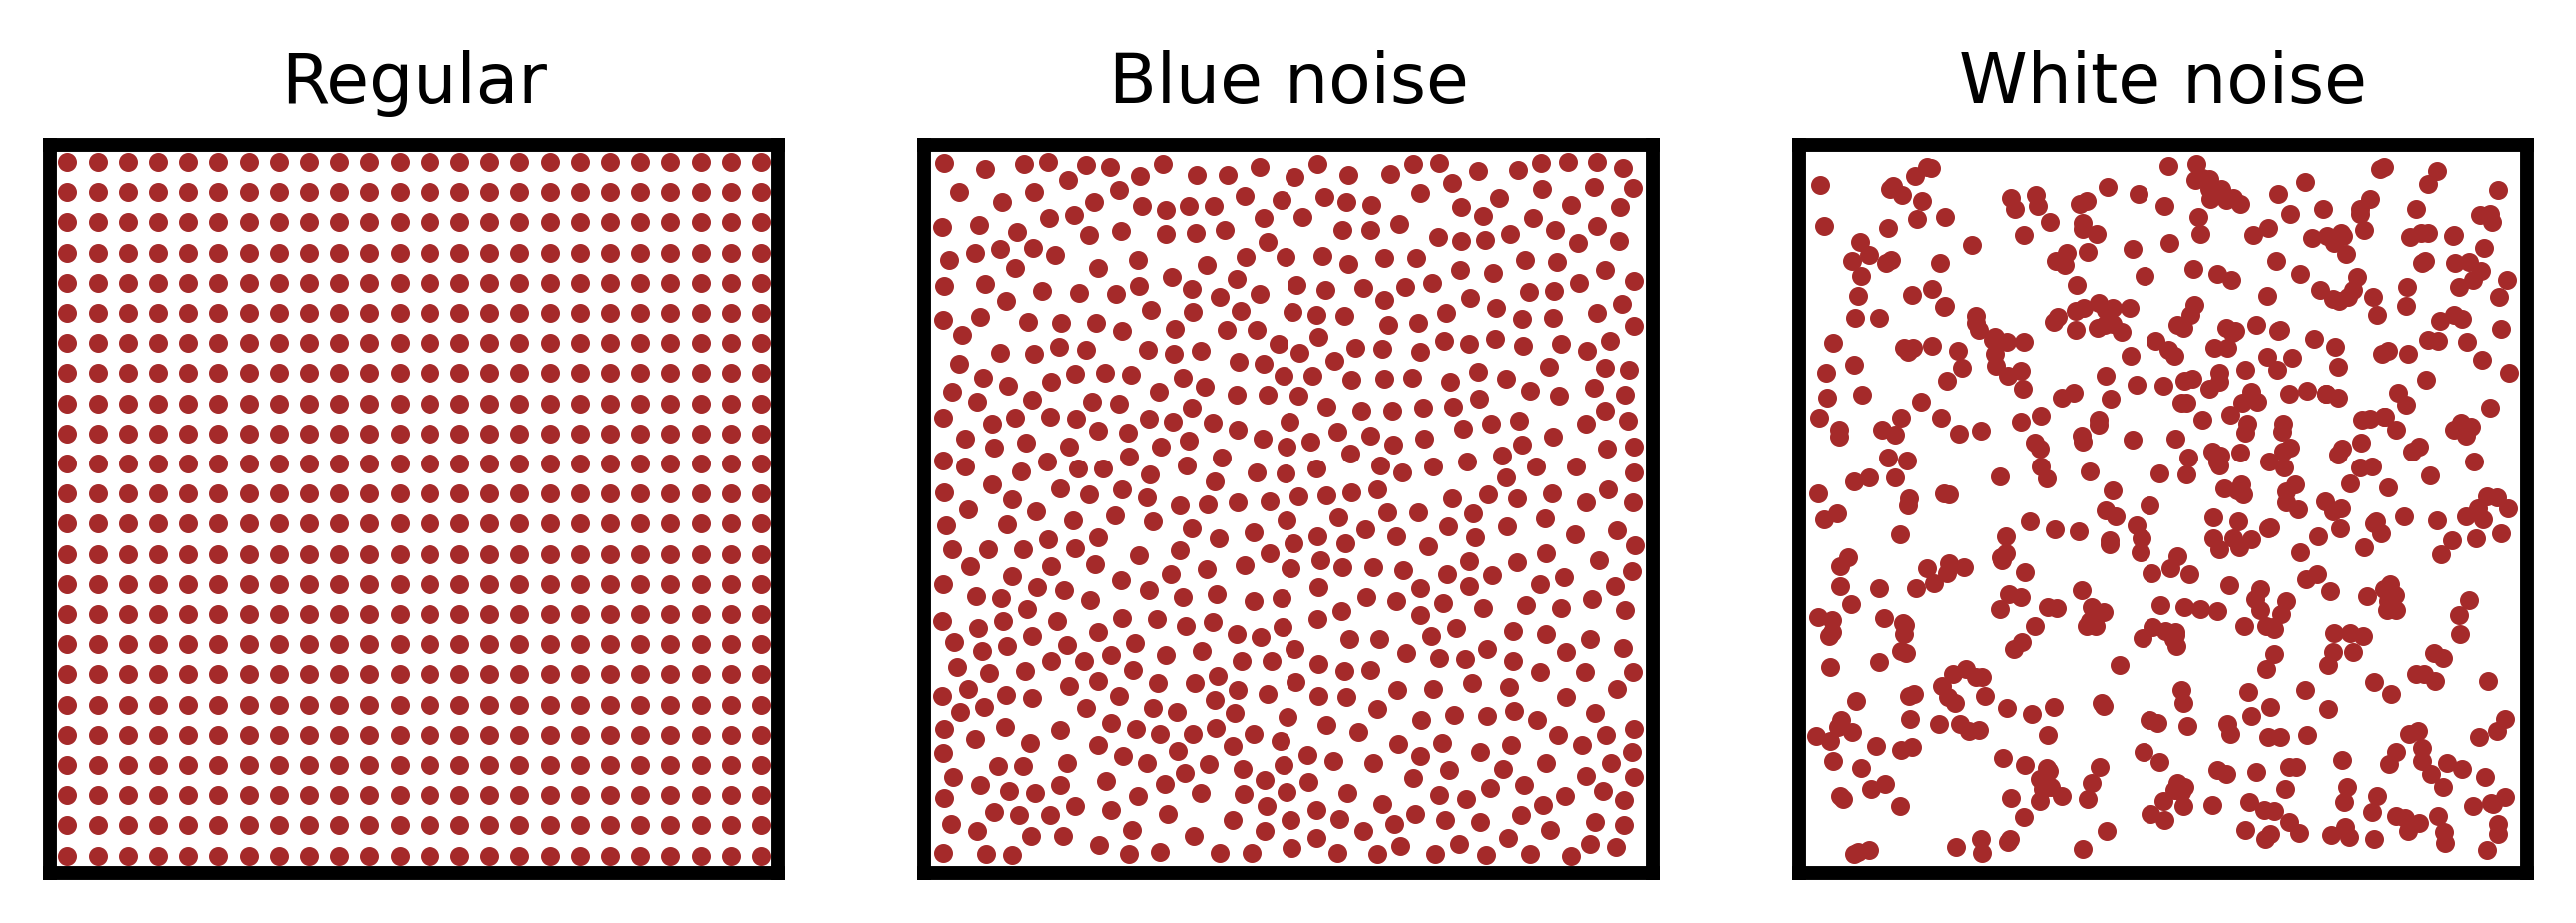
\includegraphics[width=15cm]{distribution_plot.png}
        \caption{Examples of the three kinds of input distributions. Each plot shows 24x24 inputs. Regular distribution places inputs evenly across the entire environment in a rectangular way. Noisy blue distribution gives inputs placed sequentially so each is placed as far away from other inputs as possible. White noise distribution places inputs randomly, and independent of all other inputs.}
        \label{distribution_plot}
    \end{figure}

    A set of typical parameters are shown in table 3.1, but nuances will be discussed in more detail.
    \begin{table}[H]
        \caption{Example parameters for simulations. The parameters are partially chosen for biological plausibility, and partly adapted to achieve desired firing dynamics.}
        \begin{tblr}
            {
            colspec = {X[c,h]X[c]},
            stretch = 0,
            rowsep = 6pt,
            hlines = {black, 1pt},
            vlines = {black, 1pt},
        }
        
            \textbf{Parameter} & \textbf{Value} \\
            \# Transition cells & 13\\
            \# Inputs & 576 (24x24) \\
            Theta rate & 10 Hz \\
            Phase-delay cutoff & 20 ms \\
            \(\sigma\) & 0.012 \\
            \(\mu\) & uniform[0-2] \\
            Transition cell threshold & 1.0 \\
            Transition cell \(\tau\) & 10 ms \\
            \(w_{max}\) & 0.14 \\
            \(w_{init}\) & uniform[0-0.75*\(w_{max}\)] \\
            \(A_{pre}\) & 0.01 \\
            \(A_{post}\) & -0.007 \\
            \(\tau_{pre}\) & 8 ms \\
            \(\tau_{post}\) & 80 ms \\
            Baseline & 0.005 \\
            Inhibitory delay & 0.6 ms \\
        \end{tblr}
    \end{table}

    Some of these parameters were calibrated in order to achieve a wanted dynamic. Notably, the first transition cell would ideally spike about halfway between the first input and the phase-delay cutoff, in order to facilitate STDP, and the inhibitory delay was set to encourage some other transition cells to fire, while imposing strict inhibition nonetheless. The apost, apre and baseline was set up to work in conjunction so potentiation and depression would approximately balance each other out. These parameters reflect one way of getting these dynamics to play out appropriately, and some of the models seemed to produce hexagonal transition-cells with a wider range of parameters than others.


    \printbibliography

\end{document}